
\begin{answer}
    \begin{figure}[H]
        \centering
        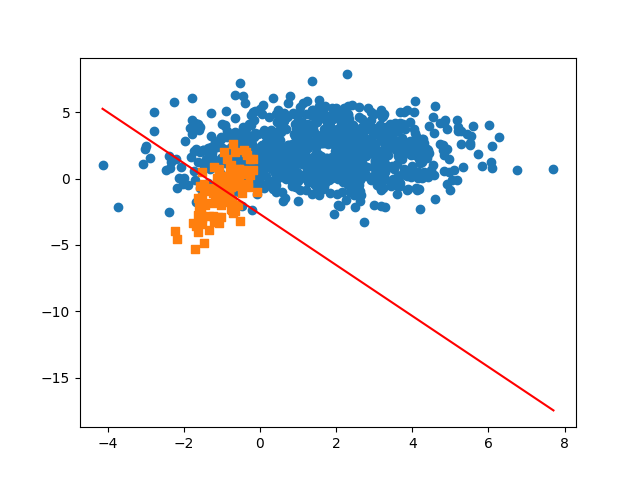
\includegraphics[width=0.6\textwidth]{src/imbalanced/imbalanced_naive_pred.png}
        \caption{Vanilla Logistic Regression on imbalanced set}
    \end{figure}

The classifiers accuracy values are the following:
\begin{verbatim}
A1: 0.57, A0: 0.975, A: 0.9381818181818181, balanced A: 0.7725
\end{verbatim}

This shows that the accuracy of positive examples is worse than the one of negative results
\end{answer}